\documentclass[a4paper,12pt]{article}

\usepackage{graphicx}
\usepackage{anysize}
\usepackage{multicol}
% USE setspace BEFORE hyperref (for footnote link)
\usepackage{setspace}
\usepackage{hyperref}
\usepackage{spverbatim}
\usepackage{enumitem}
\usepackage[top=0.5in, left=0.75in, bottom=0.5in, right=0.5in, includefoot]{geometry}
\usepackage{subcaption}
\usepackage[justification=centering]{caption}

\usepackage[compact]{titlesec}
% syntax \titlespacing{<command>}{<left>}{<before>}{<after>}
\titlespacing{\section}{0pt}{-0.5in}{*0}
\titleformat{\section}{\normalfont\fontsize{14}{22}\bfseries}{\thesection}{1em}{}

\setlength{\columnsep}{0.5cm}
\setlength{\parindent}{0pt}

\linespread{1.5}

\begin{document}

  % titlepage
  \thispagestyle{empty}
\begin{center}
  \hfill \break

  \begin{Large}
    \textbf{TRIBHUVAN UNIVERSITY}
  \end{Large}

  \begin{large}
    \textbf{INSTITUTE OF SCIENCE AND TECHNOLOGY}
  \end{large}

  \begin{normalsize}
    \textbf{Central Department of Computer Science and Information Technology}
  \end{normalsize}

  \begin{footnotesize}
    \textbf{Kirtipur, Kathmandu}\\[3cm]
  \end{footnotesize}

  
\includegraphics[width=4cm]{../tu_logo.png}\\[3cm]

Lab No.: 4

A Lab Report on \emph{\underline{Convex Hull}}\\[3cm]

  \begin{flushleft}
    \begin{multicols}{2}
      \textbf{\underline{Submitted by:}}

      Name: Brihat Ratna Bajracharya

      Roll No.: 19/075

      \hfill \break

      \textbf{\underline{Submitted to:}}

      Mr. Jagdish Bhatta

      Central Department of Computer Science and Information Technology

    \end{multicols}
  \end{flushleft}

  \hfill \break

  Date of submission: 2076 Falgun 11
\end{center}

\pagebreak


  \fontsize{14}{22}{\textbf{\underline{LAB 4}}}

  \begin{spacing}{1}
    \hfill \break
    Implement Convex Hull using
    \begin{enumerate}[leftmargin=*]
      \itemsep0em
      \item extreme points
      \item extreme edges
      \item gift wrap
      % \hfill \break
    \end{enumerate}
  \end{spacing}

  \section*{\textbf{\underline{Code}}\footnote{\url{https://github.com/Brihat9/CG/blob/master/cg_lab_4_convex_hull.py}}}

  \begin{spacing}{1}
    \begin{footnotesize}
      \begin{spverbatim}
#!/usr/bin/env python

from basics import Point, LineSegment
from circular_doubly_linked_list import CircularDoublyLinkedList
from cg_lab_3 import is_point_inclusion
from cg_lab_2_lr_turn import is_left_turn, is_colinear, compute_area

import copy
import math
import pprint

''' change input file here '''
INPUT_FILE = 'cg_lab_4_input_file_test'

def get_extreme_points_based_convex_hull(points):
    ''' returns sorted list of extreme points from given set of points
        that forms the convex hull

        parameter: points - list of points

        returns: sorted list of extreme points
    '''
    n = len(points)

    # list to add non extreme points
    non_extreme_points = []

    '''
        for i upto N - 1:
            for j != i upto N -2:
                for k != i != j upto N - 3:
                    for l != i != j != k upto N - 4:
                        if point P_l lies inside triangle(P_i, P_j, P_k):
                            P_l is non-extreme points
    '''
    for i in range(n - 1):
        for j in range(n - 2):
            if j != i:
                for k in range(n - 3):
                    if k != i and k != j:
                        for l in range(n - 4):
                            if l != i and l != j and l != k:
                                # create triangle (polygon)
                                polygon = CircularDoublyLinkedList()
                                polygon.append(points[i])
                                polygon.append(points[j])
                                polygon.append(points[k])

                                # check point_l lies inside triangle (polygon)
                                res = is_point_inclusion(polygon, points[l])

                                # if point lies inside, it is non extreme point
                                if res:
                                    non_extreme_points.append(points[l])

    ''' for testing: displays content of non_extreme_points '''
    # for index in range(len(non_extreme_points)):
    #     print(non_extreme_points[index]),
    #     print("\t"),

    ''' using python 'set' datatype to find extreme point '''
    points_set = set(points)
    non_extreme_points_set = set(non_extreme_points)
    extreme_points_set = points_set - non_extreme_points_set
    extreme_points = list(extreme_points_set)
    # print(extreme_points)

    ''' for sorting extreme points '''
    # calculate centroid of polygon
    centroid = Point(sum([point.x for point in extreme_points])/len(extreme_points),sum([point.y for point in extreme_points])/len(extreme_points))
    # print("Centroid of all Points: " + str(centroid))

    # sort vertices of polygon in anti-clockwise order
    sorted_extreme_points = copy.deepcopy(extreme_points)
    sorted_extreme_points.sort(key=lambda p: math.atan2(p.y-centroid.y,p.x-centroid.x))

    ''' for testing: show points in sorted order '''
    # print("\nExtreme points in sorted order")
    # for index in range(len(extreme_points)):
    #     print(sorted_extreme_points[index]),
    # print("\n")

    return sorted_extreme_points

def get_extreme_edges_based_convex_hull(points):
    ''' returns sorted list of extreme edges from given set of points
        that forms the convex hull

        parameter: points - list of points

        returns: sorted list of extreme edges
    '''
    n = len(points)

    # list to add non extreme points
    extreme_edges = []

    '''
        for i upto N - 1:
            for j != i upto N -2:
                for k != i != j upto N - 3:
                    if point P_k is left or colinear with line(P_i, P_j):
                         line(P_i, P_j) is extreme edge
                     else:
                         line(P_i, P_j) is non-extreme edge
    '''
    for i in range(n):
        for j in range(n):
            if j != i:
                res = [None] * n
                line = LineSegment(points[i], points[j])
                for k in range(n):
                    res[k] = is_left_turn(points[i], points[j], points[k]) or is_colinear(points[i], points[j], points[k])
                if set(res) == {True}:
                    ''' for test '''
                    # print(points[i]),; print("\t"),; print(points[j]),; print("\t"),; print(res)

                    extreme_edges.append(line)

    # print(extreme_edges)
    extreme_edges_set = set(extreme_edges)

    ''' get vertices from extreme edges '''
    extreme_edge_vertex = []
    for index in range(len(extreme_edges)):
        line = extreme_edges[index]
        extreme_edge_vertex.append(line.start)
        extreme_edge_vertex.append(line.terminal)

    ''' get unique vertices from extreme edge vertices '''
    eev = list(set(extreme_edge_vertex))
    # print(eev)

    ''' for testing: displays content of non_extreme_points '''
    # for index in range(len(eev)):
    #     print(eev[index]),
    #     print("\t"),

    ''' for sorting extreme edge vertices '''
    centroid = Point(sum([point.x for point in eev])/len(eev),sum([point.y for point in eev])/len(eev))

    sorted_eev = copy.deepcopy(eev)
    sorted_eev.sort(key=lambda p: math.atan2(p.y-centroid.y,p.x-centroid.x))

    ''' for testing only '''
    # for index in range(len(sorted_eev)):
    #     print(sorted_eev[index]),
    #     print("\t"),

    ''' obtain sorted edges from sorted edge vertices '''
    sorted_edge = []

    num_sorted_vertices = len(sorted_eev)
    for index in range(num_sorted_vertices):
        edge = LineSegment(sorted_eev[index], sorted_eev[(index + 1) % num_sorted_vertices])
        sorted_edge.append(edge)

    ''' for testing only: sorted edges '''
    # for index in range(len(sorted_edge)):
    #     print(sorted_edge[index]),
    #     print("\t"),

    return(sorted_edge)

def gift_wrap_convex_hull_linked_list(point_linked_list):
    ''' Gift Wrap Algorithm implementation using Circular Doubly Linked List

        parameter: point_linked_list = Circular Doubly Linked List of sorted
                   points (in non decreasing order of Y-Coord)

        result: Circular Doubly Linked List of Convex Hull Points
    '''

    # result to return
    gift_wrap_linked_list = CircularDoublyLinkedList()

    # first point is the point with least Y- coordinate
    first_point = point_linked_list.head

    # take first point as reference, and set next point to None '''
    ref_point = first_point
    next_point = None

    while(True):
        # add reference point to result
        gift_wrap_linked_list.append(ref_point.data)

        # get next point in linked list
        next_point = ref_point.next

        # set cursor to head of linked list
        cursor = point_linked_list.head

        # for all node in linked list
        while(True):
            # if there exist a point counter-clockwise to next point, set that point as next point
            if(compute_area(ref_point.data, cursor.data, next_point.data) > 0.0):
                next_point = cursor

            # increment cursor to next node
            cursor = cursor.next

            # stop when cursor reach head of linked list again
            if(cursor == point_linked_list.head):
                break

        # set next point as reference point for next iteration
        ref_point = next_point

        # iterate until we reach head of linked list
        if(ref_point == point_linked_list.head):
            break

    return gift_wrap_linked_list

def graham_scan_convex_hull(points):
    ''' Graham Scan Algorithm

        parameter: points = array of given points

        result: Array of Convex Hull Points
    '''

    # num of points
    vertex_num = len(points)

    # if number of points are less than 4, then the input set of points
    # are the convex hull itself
    if vertex_num < 4:
        return points

    # result variable
    convex_hull_graham_scan = []

    # get min Y- Coord point
    sorted_points_inc_y = copy.deepcopy(points)
    sorted_points_inc_y.sort(key=lambda p: p.y)
    min_y_coord_point = sorted_points_inc_y[0]
    # print(min_y_coord_point)

    # sort points in anti-clockwise order wrt min_y_coord_point
    sorted_p = copy.deepcopy(points)
    sorted_p.sort(key=lambda p: math.atan2(p.y-min_y_coord_point.y,p.x-min_y_coord_point.x))

    ''' Graham Scan Algorithm begins here '''
    # add first three coordinates of sorted points in result
    convex_hull_graham_scan.append(sorted_p[0])
    convex_hull_graham_scan.append(sorted_p[1])
    convex_hull_graham_scan.append(sorted_p[2])

    ''' these are top of stack and next top of stack, using list (for testing)'''
    # print(point_stack[-1])
    # print(point_stack[-2])

    '''
        i = 3
        while(i < N):
            if left_turn(top(stack), next_top(stack), sorted_point(i)):
                stack.push(sorted_point[i])
                i++
            else:
                stack.pop()
    '''
    index = 3
    while(index < vertex_num):
        if is_left_turn(convex_hull_graham_scan[-2], convex_hull_graham_scan[-1], sorted_p[index]):
            convex_hull_graham_scan.append(sorted_p[index])
            index += 1
        else:
            convex_hull_graham_scan.pop()

    return convex_hull_graham_scan

def main():
    """ Main Function """

    print("CG LAB 4")
    print("Brihat Ratna Bajracharya\n19/075\n")

    ''' reads input file '''
    in_file = open(INPUT_FILE, 'r')

    ''' get number of points '''
    print("Enter number of points:"),
    points_num = int(in_file.readline())
    print(points_num)

    ''' reads coords of point '''
    input_coords = in_file.readline()
    input_coords_list = input_coords.split()
    # print(input_coords_list)

    ''' initialize vertex list '''
    points = [None] * points_num

    ''' get coordinates of each point '''
    for index in range(points_num):
        print(" Enter coordinates of point P{}:".format(index+1)),
        input_coords_point = input_coords_list[index].split(',')
        points[index] = Point(int(input_coords_point[0]), int(input_coords_point[1]))
        print(points[index])

    ''' FINDING CONVEX HULL BASED ON EXTREME POINTS '''
    convex_hull_exp_pt = get_extreme_points_based_convex_hull(points)

    print("\nConvex Hull (Extreme Points): ["),
    for index in range(len(convex_hull_exp_pt)):
        print(convex_hull_exp_pt[index]),
        if index != len(convex_hull_exp_pt) - 1:
            print(","),
    print("]")

    ''' FINDING CONVEX HULL BASED ON EXTREME EDGES '''
    convex_hull_exp_edges = get_extreme_edges_based_convex_hull(points)

    print("\nConvex Hull (Extreme Edges): ["),
    for index in range(len(convex_hull_exp_edges)):
        print(convex_hull_exp_edges[index]),
        if index != len(convex_hull_exp_edges) - 1:
            print("---"),
    print("]")

    ''' FINDING CONVEX HULL: GIFT WRAP ALGORITHM (USING CIRCULAR DOUBLY LINKED LIST) '''
    points_inc_order_of_y_coord = copy.deepcopy(points)
    points_inc_order_of_y_coord.sort(key=lambda point: point.y)

    point_linked_list = CircularDoublyLinkedList()

    for index in range(len(points)):
        point_linked_list.append(points_inc_order_of_y_coord[index])

    convex_hull_gift_wrap_linked_list = gift_wrap_convex_hull_linked_list(point_linked_list)
    convex_hull_gift_wrap_linked_list.display("Convex Hull (Gift Wrap) 2")

    ''' FINDING CONVEX HULL: GRAHAM SCAN ALGORITHM '''
    convex_hull_graham_scan = graham_scan_convex_hull(points)

    print("\nConvex Hull (Graham Scan): ["),
    for index in range(len(convex_hull_graham_scan)):
        print(convex_hull_graham_scan[index]),
        if index != len(convex_hull_graham_scan) - 1:
            print(","),
    print("]")

    print("\nDONE.")

if __name__ == '__main__':
    main()
      \end{spverbatim}
    \end{footnotesize}
  \end{spacing}

  \section*{\textbf{\underline{Output}}}
  \begin{spacing}{1}
    \begin{footnotesize}
      \begin{spverbatim}
$ ./cg_lab_4_convex_hull.py

CG LAB 4
Brihat Ratna Bajracharya
19/075

Enter number of points: 11
 Enter coordinates of point P1: (5, 8)
 Enter coordinates of point P2: (2, 7)
 Enter coordinates of point P3: (7, 7)
 Enter coordinates of point P4: (5, 6)
 Enter coordinates of point P5: (3, 5)
 Enter coordinates of point P6: (6, 5)
 Enter coordinates of point P7: (4, 4)
 Enter coordinates of point P8: (3, 3)
 Enter coordinates of point P9: (2, 2)
 Enter coordinates of point P10: (5, 2)
 Enter coordinates of point P11: (8, 3)

Convex Hull (Extreme Points): [ (3, 3) , (2, 2) , (5, 2) , (8, 3) , (7, 7) , (5, 8) , (2, 7) ]

Convex Hull (Extreme Edges): [ [(2, 2), (5, 2)] --- [(5, 2), (8, 3)] --- [(8, 3), (7, 7)] --- [(7, 7), (5, 8)] --- [(5, 8), (2, 7)] --- [(2, 7), (2, 2)] ]

Convex Hull (Gift Wrap) 2: [ (2, 2) (5, 2) (8, 3) (7, 7) (5, 8) (2, 7) ] #
Convex Hull (Graham Scan): [ (2, 2) , (5, 2) , (8, 3) , (7, 7) , (5, 8) , (2, 7) ]
DONE.
      \end{spverbatim}
    \end{footnotesize}
  \end{spacing}

  \begin{figure}[h!]
    \centering
    \begin{subfigure}[b]{0.2\linewidth}
      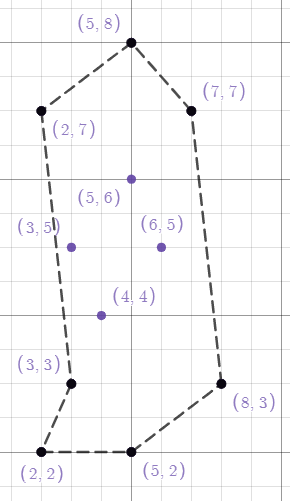
\includegraphics[width=\linewidth]{cg_lab_4_output_extreme_points.png}
      \caption{Using \\Extreme Points}
    \end{subfigure}
    \hspace{1in}
    \begin{subfigure}[b]{0.2\linewidth}
      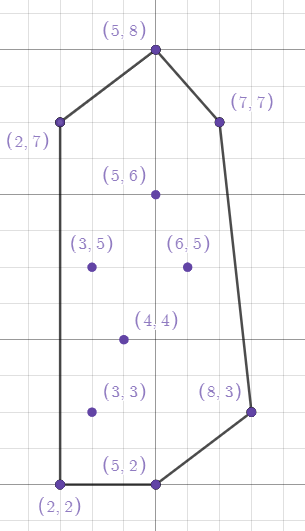
\includegraphics[width=\linewidth]{cg_lab_4_output_extreme_edges.png}
      \caption{Using \\Extreme Edge}
    \end{subfigure}
    \hspace{1in}
    \begin{subfigure}[b]{0.2\linewidth}
      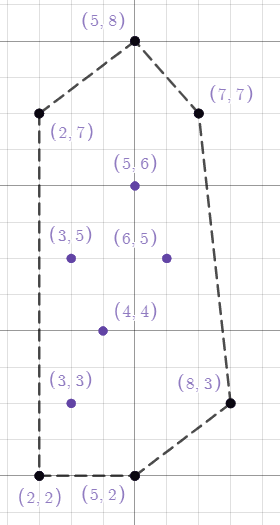
\includegraphics[width=\linewidth]{cg_lab_4_output_gift_wrap.png}
      \caption{Using \\Gift Wrap/Graham Scan}
    \end{subfigure}
    \caption{Convex Hull}
    \label{fig:convex_hull}
  \end{figure}

  \vspace{1cm}

  \section*{\textbf{\underline{Input File}}\footnote{\url{https://github.com/Brihat9/CG/blob/master/cg_lab_4_input_file}}}
  \begin{spacing}{1}
    \begin{footnotesize}
      \begin{spverbatim}
11
5,8 2,7 7,7 5,6 3,5 6,5 4,4 3,3 2,2 5,2 8,3
      \end{spverbatim}
    \end{footnotesize}
  \end{spacing}

\end{document}
